\documentclass[11pt]{article}

% Change "review" to "final" to generate the final (sometimes called camera-ready) version.
% Change to "preprint" to generate a non-anonymous version with page numbers.
\usepackage[review]{acl}

% Standard package includes
\usepackage{times}
\usepackage{latexsym}

% For proper rendering and hyphenation of words containing Latin characters (including in bib files)
\usepackage[T1]{fontenc}
% For Vietnamese characters
% \usepackage[T5]{fontenc}
% See https://www.latex-project.org/help/documentation/encguide.pdf for other character sets

% This assumes your files are encoded as UTF8
\usepackage[utf8]{inputenc}

% This is not strictly necessary, and may be commented out,
% but it will improve the layout of the manuscript,
% and will typically save some space.
\usepackage{microtype}

% This is also not strictly necessary, and may be commented out.
% However, it will improve the aesthetics of text in
% the typewriter font.
\usepackage{inconsolata}

%Including images in your LaTeX document requires adding
%additional package(s)
\usepackage{graphicx}
\usepackage{hyperref}
\usepackage{cleveref}
\usepackage{todonotes}
\usepackage{booktabs}
\newcommand{\ie}{\textit{i.e.,}\@\xspace}

% All figures live in the repo's top-level figures/ directory (one level up
% from paper/), generated by the scripts in figures/*.py -- not copied here.
\graphicspath{{../figures/}}

% Source - https://tex.stackexchange.com/a/161760
% Posted by Mico, modified by community. See post 'Timeline' for change history
% Retrieved 2026-07-15, License - CC BY-SA 3.0

%\setcounter{topnumber}{8}
%\setcounter{bottomnumber}{8}
%\setcounter{totalnumber}{8}


% If the title and author information does not fit in the area allocated, uncomment the following
%
%\setlength\titlebox{<dim>}
%
% and set <dim> to something 5cm or larger.

\title{Are Latent Reasoning Tokens Unnecessary for Model Performance?}

% Author information can be set in various styles:
% For several authors from the same institution:
% \author{Author 1 \and ... \and Author n \\
%         Address line \\ ... \\ Address line}
% if the names do not fit well on one line use
%         Author 1 \\ {\bf Author 2} \\ ... \\ {\bf Author n} \\
% For authors from different institutions:
% \author{Author 1 \\ Address line \\  ... \\ Address line
%         \And  ... \And
%         Author n \\ Address line \\ ... \\ Address line}
% To start a separate ``row'' of authors use \AND, as in
% \author{Author 1 \\ Address line \\  ... \\ Address line
%         \AND
%         Author 2 \\ Address line \\ ... \\ Address line \And
%         Author 3 \\ Address line \\ ... \\ Address line}

\author{Austin Long \\
  Institute for Safe Autonomy \\
  University of York \\
  \texttt{austin.long@york.ac.uk} \\\And
  Colin Paterson \\
  Institute for Safe Autonomy \\
  University of York \\
  \texttt{colin.paterson@york.ac.uk} \\\And
  Jing Xu \\
  Institute for Safe Autonomy \\
  University of York \\
  \texttt{jing.xu@york.ac.uk} \\}

%\author{
%  \textbf{First Author\textsuperscript{1}},
%  \textbf{Second Author\textsuperscript{1,2}},
%  \textbf{Third T. Author\textsuperscript{1}},
%  \textbf{Fourth Author\textsuperscript{1}},
%\\
%  \textbf{Fifth Author\textsuperscript{1,2}},
%  \textbf{Sixth Author\textsuperscript{1}},
%  \textbf{Seventh Author\textsuperscript{1}},
%  \textbf{Eighth Author \textsuperscript{1,2,3,4}},
%\\
%  \textbf{Ninth Author\textsuperscript{1}},
%  \textbf{Tenth Author\textsuperscript{1}},
%  \textbf{Eleventh E. Author\textsuperscript{1,2,3,4,5}},
%  \textbf{Twelfth Author\textsuperscript{1}},
%\\
%  \textbf{Thirteenth Author\textsuperscript{3}},
%  \textbf{Fourteenth F. Author\textsuperscript{2,4}},
%  \textbf{Fifteenth Author\textsuperscript{1}},
%  \textbf{Sixteenth Author\textsuperscript{1}},
%\\
%  \textbf{Seventeenth S. Author\textsuperscript{4,5}},
%  \textbf{Eighteenth Author\textsuperscript{3,4}},
%  \textbf{Nineteenth N. Author\textsuperscript{2,5}},
%  \textbf{Twentieth Author\textsuperscript{1}}
%\\
%\\
%  \textsuperscript{1}Affiliation 1,
%  \textsuperscript{2}Affiliation 2,
%  \textsuperscript{3}Affiliation 3,
%  \textsuperscript{4}Affiliation 4,
%  \textsuperscript{5}Affiliation 5
%\\
%  \small{
%    \textbf{Correspondence:} \href{mailto:email@domain}{email@domain}
%  }
%}

\begin{document}
\maketitle
\begin{abstract}
Training large language models to perform latent reasoning may improve performance, but the lack of legible reasoning poses challenges for model interpretability and safety assurance. This challenge has motivated interpretability research that aims to characterise the functional role of latent reasoning tokens. Some studies indicate that latent reasoning tokens are effective, whereas other work suggests that these tokens are under-utilised. In this paper, we consider the tension between existing findings by reproducing prior work which shows that some latent reasoning tokens are not necessary. 
Two interesting observations emerge from our experiments. First, we find that latent reasoning models often generate redundant tokens due to the fixed token budgets. Second, we observe that explicit reasoning models fine-tuned on gold reasoning traces may copy the result of the most recent reasoning step when generating an answer. 
% By performing targeted ablations, we identify two factors that affect the interpretation of these results: 1) fixed token budgets force latent reasoning models to generate redundant tokens, 2) explicit reasoning models fine-tuned on gold reasoning traces may learn to copy the result of the most recent reasoning step when generating an answer.
\end{abstract}

\section{Introduction}

Large language models (LLMs) have become increasingly central to AI research as their capabilities have been improved by scale~\cite{kaplan2020scaling}. These capabilities are especially pronounced in explicit reasoning models (ERMs), such as OpenAI o1~\cite{jaech2024openai} and DeepSeek R1~\cite{guo2025deepseek}, that learn to produce higher quality outputs by starting their responses with a chain-of-thought (CoT): a passage of text in which the model's given task is broken down into smaller steps that can be tackled one at a time \cite{wei2022chain}. Latent reasoning models (LRMs), such as COCONUT \cite{hao2024training} and CODI \cite{shen2025codi}, replace these human-readable steps with an illegible array of numbers, as shown in~\Cref{fig:Comparison}. This modification may improve reasoning performance, but it also raises new challenges for our understanding of these systems.

\begin{figure}[h]
  \centering
  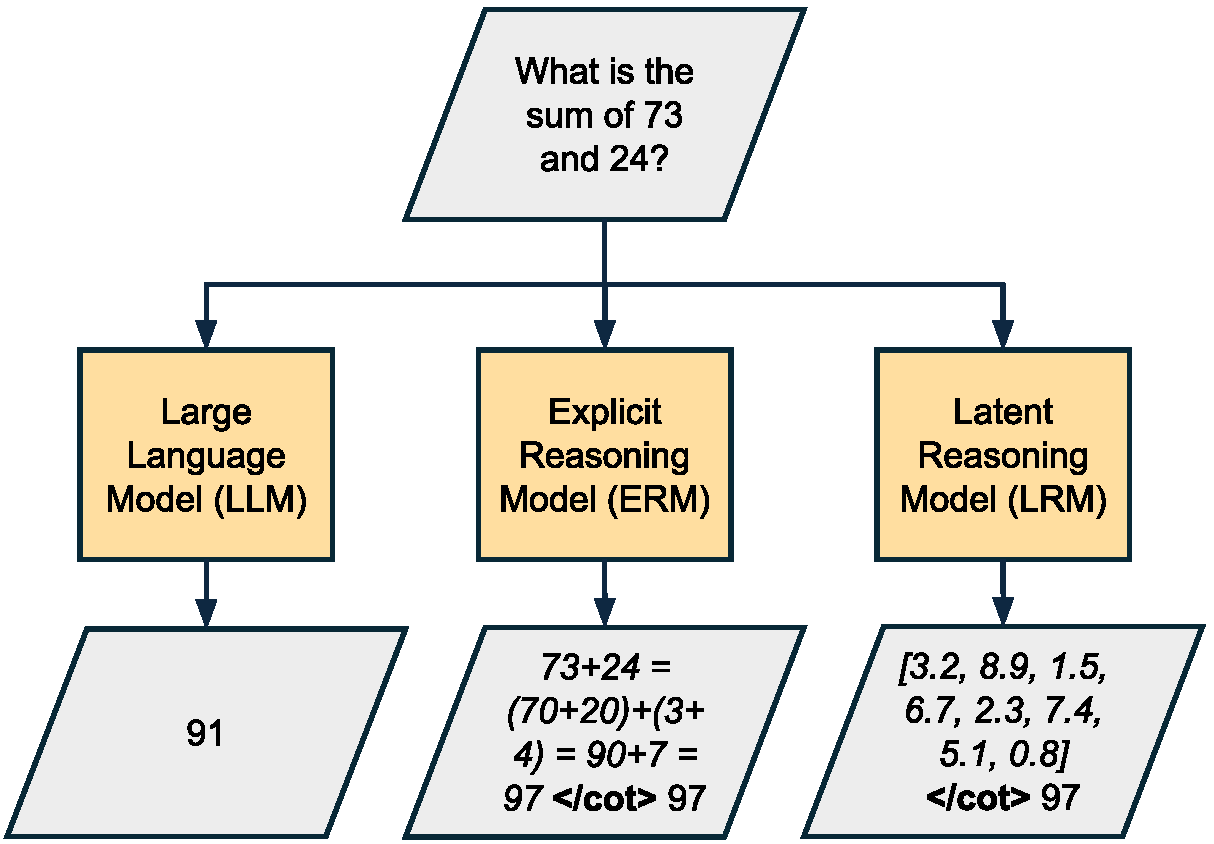
\includegraphics[width=0.9\columnwidth]{LRM_Comparison.pdf}
  \caption{\textbf{A comparison of model outputs.}}
  \label{fig:Comparison}
\end{figure}

% \Description{The prompt "What is the sum of 73 and 24?" is fed into three models. The first is a large language model, and it is shown to respond with "91". The second is an explicit reasoning model, and it is shown to respond with a chain-of-thought "73+24 = (70+20)+(2+4) = 90+7 = 97", followed by a delimiter, "</cot>", followed by an answer, "97". The final model is a latent reasoning model, that is shown to respond to the prompt with a vector of numbers, "[3.2, 8.9, 1.5, 6.7, 2.3, 7.4, 5.1, 0.8]", followed by the same delimiter used by the explicit reasoning model, and the answer "97".}

Interpreting LLMs is difficult due to complications like polysemanticity and superposition \cite{olah2020zoom, elhage2022toy}. However, explicit CoTs have proved advantageous, as they can provide observers with information about model reasoning. This information can be leveraged to improve model safeguards, such as monitoring systems, as shown by \citet{baker2025monitoring}. \citet{korbak2025chain} warn that these advantages could be lost in the transition to latent reasoning.

Work on interpreting latent reasoning models has been motivated by a need to address these risks. Some research has attempted to decode latent reasoning tokens \cite{shen2025codi}, or replace them with a legible representations \cite{wang2026beyond}. Other studies attempt to characterise the functional role of latent reasoning tokens. \citet{hao2024training} show that COCONUT uses its latent CoT to attempt multiple solutions in parallel, while \citet{goyal2025scratchpad} show that CODI's confidence in the correct answer gradually increases as additional latent reasoning tokens are generated. In contrast, \citet{dilgren2026latent} show that some LRMs may determine their final answer before generating part or all of their CoT. In this paper, we aim to address the tension between these findings.

The rest of the paper is structured as follows, in Section~\ref{sec:experiment} we replicate the experiment performed by \citet{dilgren2026latent}. We proceed by performing ablations to understand the factors contributing to the discrepancy between the results reported for COCONUT, CODI, and the ERM. We identify two factors that contribute to this discrepancy: the first is the fixed token budgets used by the LRMs (Section~\ref{sec:difficulty}), which force them to generate redundant latent reasoning tokens; the second is the tendency of the ERM to copy the result of the most recent explicit reasoning step when generating an answer (Section~\ref{sec:copying}), which inflates perceived reasoning step necessity since truncating the CoT often causes the ERM to change its answer.

\section{Background}

\paragraph{Latent Reasoning Models:} Latent reasoning models work by applying recurrent computations to the final hidden state. Two distinct categories of latent reasoning models can be identified: vertical recurrence models, such as Huginn-0125 \cite{geiping2026scaling} and Ouro \cite{zhu2025scaling}, that repeatedly apply intermediate layers in a deep neural network to the final hidden state; and horizontal recurrence models, such as Switch \cite{yang2026demystifying} and SIM-CoT \cite{wei2025sim}, that generate latent reasoning through an autoregressive process where the final hidden state is combined with the prompt and used as input to another forward pass. In this paper, we focus on two horizontal-recurrence-based latent reasoning models: COCONUT \cite{hao2024training} and CODI \cite{shen2025codi}.

% \cite{hao2024training} which is a training procedure that produces latent reasoning models by applying a training curriculum to a base model. First, the model is fine-tuned on a dataset of explicit reasoning traces. Then, an iterative approach is used to replace one explicit reasoning step at a time with latent reasoning \cite{hao2024training}.

\paragraph{Latent Reasoning Interpretability:} Existing work has commented on whether or not latent reasoning tokens are necessary for model performance, but conclusions appear to be mixed. \citet{wang2026beyond} show that features in sparse latent reasoning tokens are causally effective operators. \citet{li_dynamics_2026} find that some latent reasoning tokens have an outsized causal influence on the model's final answer, while some aren't as effective, and that a correct answer can often be decoded early. Similarly, \citet{aswal_observable_2026} also show that the causal effect of latent reasoning tokens on the model's final answer is varied, and \citet{chang_unlocking_2026} find that early latent reasoning tokens act as critical causal hubs. \citet{goyal2025scratchpad} investigate a mechanism that may explain the heterogeneity in CODI. 
It is shown that interventions on even latent reasoning tokens, which appear to store information, are more impactful than interventions on odd latent reasoning tokens, which appear to be transitional states produced during computation over that stored information. \citet{cui_how_2026} report pervasive "shortcut" behaviour, where LRMs perform well without utilising their latent reasoning tokens. \citet{viveiros_whats_2026} examines visual LRMs and produce similar results, finding that performance wasn't significantly different when reasoning tokens were swapped out for dummy tokens. \citet{jin_final_2026} show that the necessity of latent reasoning tokens can change during the course of training. Our work focuses particularly on \citet{dilgren2026latent}, who find that truncating the latent CoT often doesn't change the models answer, and conclude that latent reasoning tokens may not be necessary for model performance.

% Some existing interpretability work on latent reasoning models has commented on the functional role of latent reasoning tokens. \citet{shen2025codi} decode latent reasoning tokens by applying the logit lens alongside attention analysis methods. The decoded latent reasoning tokens reveal a surprising pattern, which \citet{goyal2025scratchpad} explained as an alternation between stored intermediate results, and transitional states produced during computations over those stored results. \citet{dilgren2026latent} apply similar methods when decoding latent reasoning tokens generated by COCONUT and CODI. They find that latent reasoning tokens can be used to reconstruct gold reasoning traces. However, they also terminate the generation of latent reasoning, by inserting the special \verb|<eot>| token prematurely, and find that the model's answer often doesn't change. We replicate this experiment in section \ref{sec:experiment}, and proceed to provide further analysis.

\begin{table*}[]
  \centering
  \begin{tabular}{l cc cc cc}
    \hline
    & \multicolumn{2}{c}{\textbf{GSM8k}} & \multicolumn{2}{c}{\textbf{ProsQA}} & \multicolumn{2}{c}{\textbf{PrOntoQA}} \\
    \cline{2-3} \cline{4-5} \cline{6-7}
    \textbf{Model} & \textbf{Ours} & \textbf{D\&W} & \textbf{Ours} & \textbf{D\&W} & \textbf{Ours} & \textbf{D\&W} \\
    \hline
    ERM        & 41.5\%       & 41.6\%       & 74.2\% & 74.2\% & 99.2\% & 99.3\% \\
    COCONUT    & 33.1\%       & 33.1\%       & 93.8\% & 98.0\% & 98.9\% & 99.0\% \\
    CODI       & 41.6\%   & 42.2\%   & 81.4\% & 81.6\% & 94.9\% & 95.1\% \\
    \hline
  \end{tabular}
  \caption{\textbf{Testing accuracy of explicit reasoning model and two latent reasoning models (COCONUT, CODI) on three datasets.} D \& W defines the corresponding score reported by \citet{dilgren2026latent}.}
  \label{tab:performance}
\end{table*}

\section{Reproduction}
\label{sec:experiment}

We reproduce the experimental setup described by \citet{dilgren2026latent}, which aims to determine the extent to which reasoning tokens are necessary for model performance. Problems are sampled from a dataset and given to a reasoning model, which generates a response to each problem. A model's response is comprised of a CoT, which consists of reasoning tokens, and the model's final answer. Several truncated versions of the CoT are created by removing all reasoning tokens after a given point. The model is prefilled with the problem statement and each truncated CoT, and then forced to generate an answer as we terminate the CoT by inserting an \verb|<eot>| token. The resulting answers are compared to the model's original answer to determine the impact of the removed reasoning. In the rest of this section we provide additional details on the experimental setup.

% \footnote{Code available at \hyperlink{https://github.com/Aauustiin/lrm-early-stoppage-replication}{https://github.com/Aauustiin/lrm-early-stoppage-replication}}

\paragraph{Datasets:} We use the same 3 datasets as \citet{dilgren2026latent}: GSM8k \cite{cobbe2021training}, ProsQA \cite{hao2024training}, and PrOntoQA \cite{saparov2022language}. GSM8k consists of numerical math problems solvable by "a bright middle school student", whereas both ProsQA and PrOntoQA consist of logic problems. All instances from each dataset include a problem statement, an answer, and an exemplar reasoning trace. Examples are provided in Appendix~\ref{sec:appendix-examples}. Each dataset is split into a training partition, which is used to fine-tune our models, and a testing partition. More details on dataset partitions are provided in Appendix~\ref{sec:appendix-splits}.

\paragraph{Models:} We evaluate the same three models used by \citet{dilgren2026latent}, all of which are trained by fine-tuning GPT-2 small \cite{radford2019language}. The first model is an ERM trained by fine-tuning on exemplar reasoning traces. The second and third models have latent reasoning capabilities, and are trained by applying the COCONUT \citep{hao2024training} and CODI \citep{shen2025codi} training procedures. We do not train these models ourselves, but instead use the checkpoints provided by the original authors.\footnote{\hyperlink{https://huggingface.co/collections/connordilgren/are-latent-reasoning-models-easily-interpretable}{https://huggingface.co/collections/connordilgren/are-latent-reasoning-models-easily-interpretable}, \hyperlink{https://huggingface.co/zen-E/CODI-gpt2}{https://huggingface.co/zen-E/CODI-gpt2}} In Table~\ref{tab:performance} we show that these checkpoints produce similar accuracy scores as those reported by \citet{dilgren2026latent}.

\paragraph{Metrics:} We compute the two metrics described by \citet{dilgren2026latent}. The first is \emph{first match}, which is equal to the minimum number of reasoning tokens that must be generated before a model first produces the same answer as it would have if it had finished generating its CoT. The second metric is \emph{stable match}, which is equal to the minimum number of reasoning tokens after which the model does not change its answer regardless of the number of additional tokens remaining. In line with \citet{dilgren2026latent}, we divide first match and stable match by the number of latent reasoning tokens or explicit reasoning steps in the corresponding CoT and report the fraction as the result. In~\Cref{fig:replication} we show that our reproduction achieves similar matching metrics as \citet{dilgren2026latent}, we expect that differences are the result of run-to-run variation.

\begin{figure*}[]
  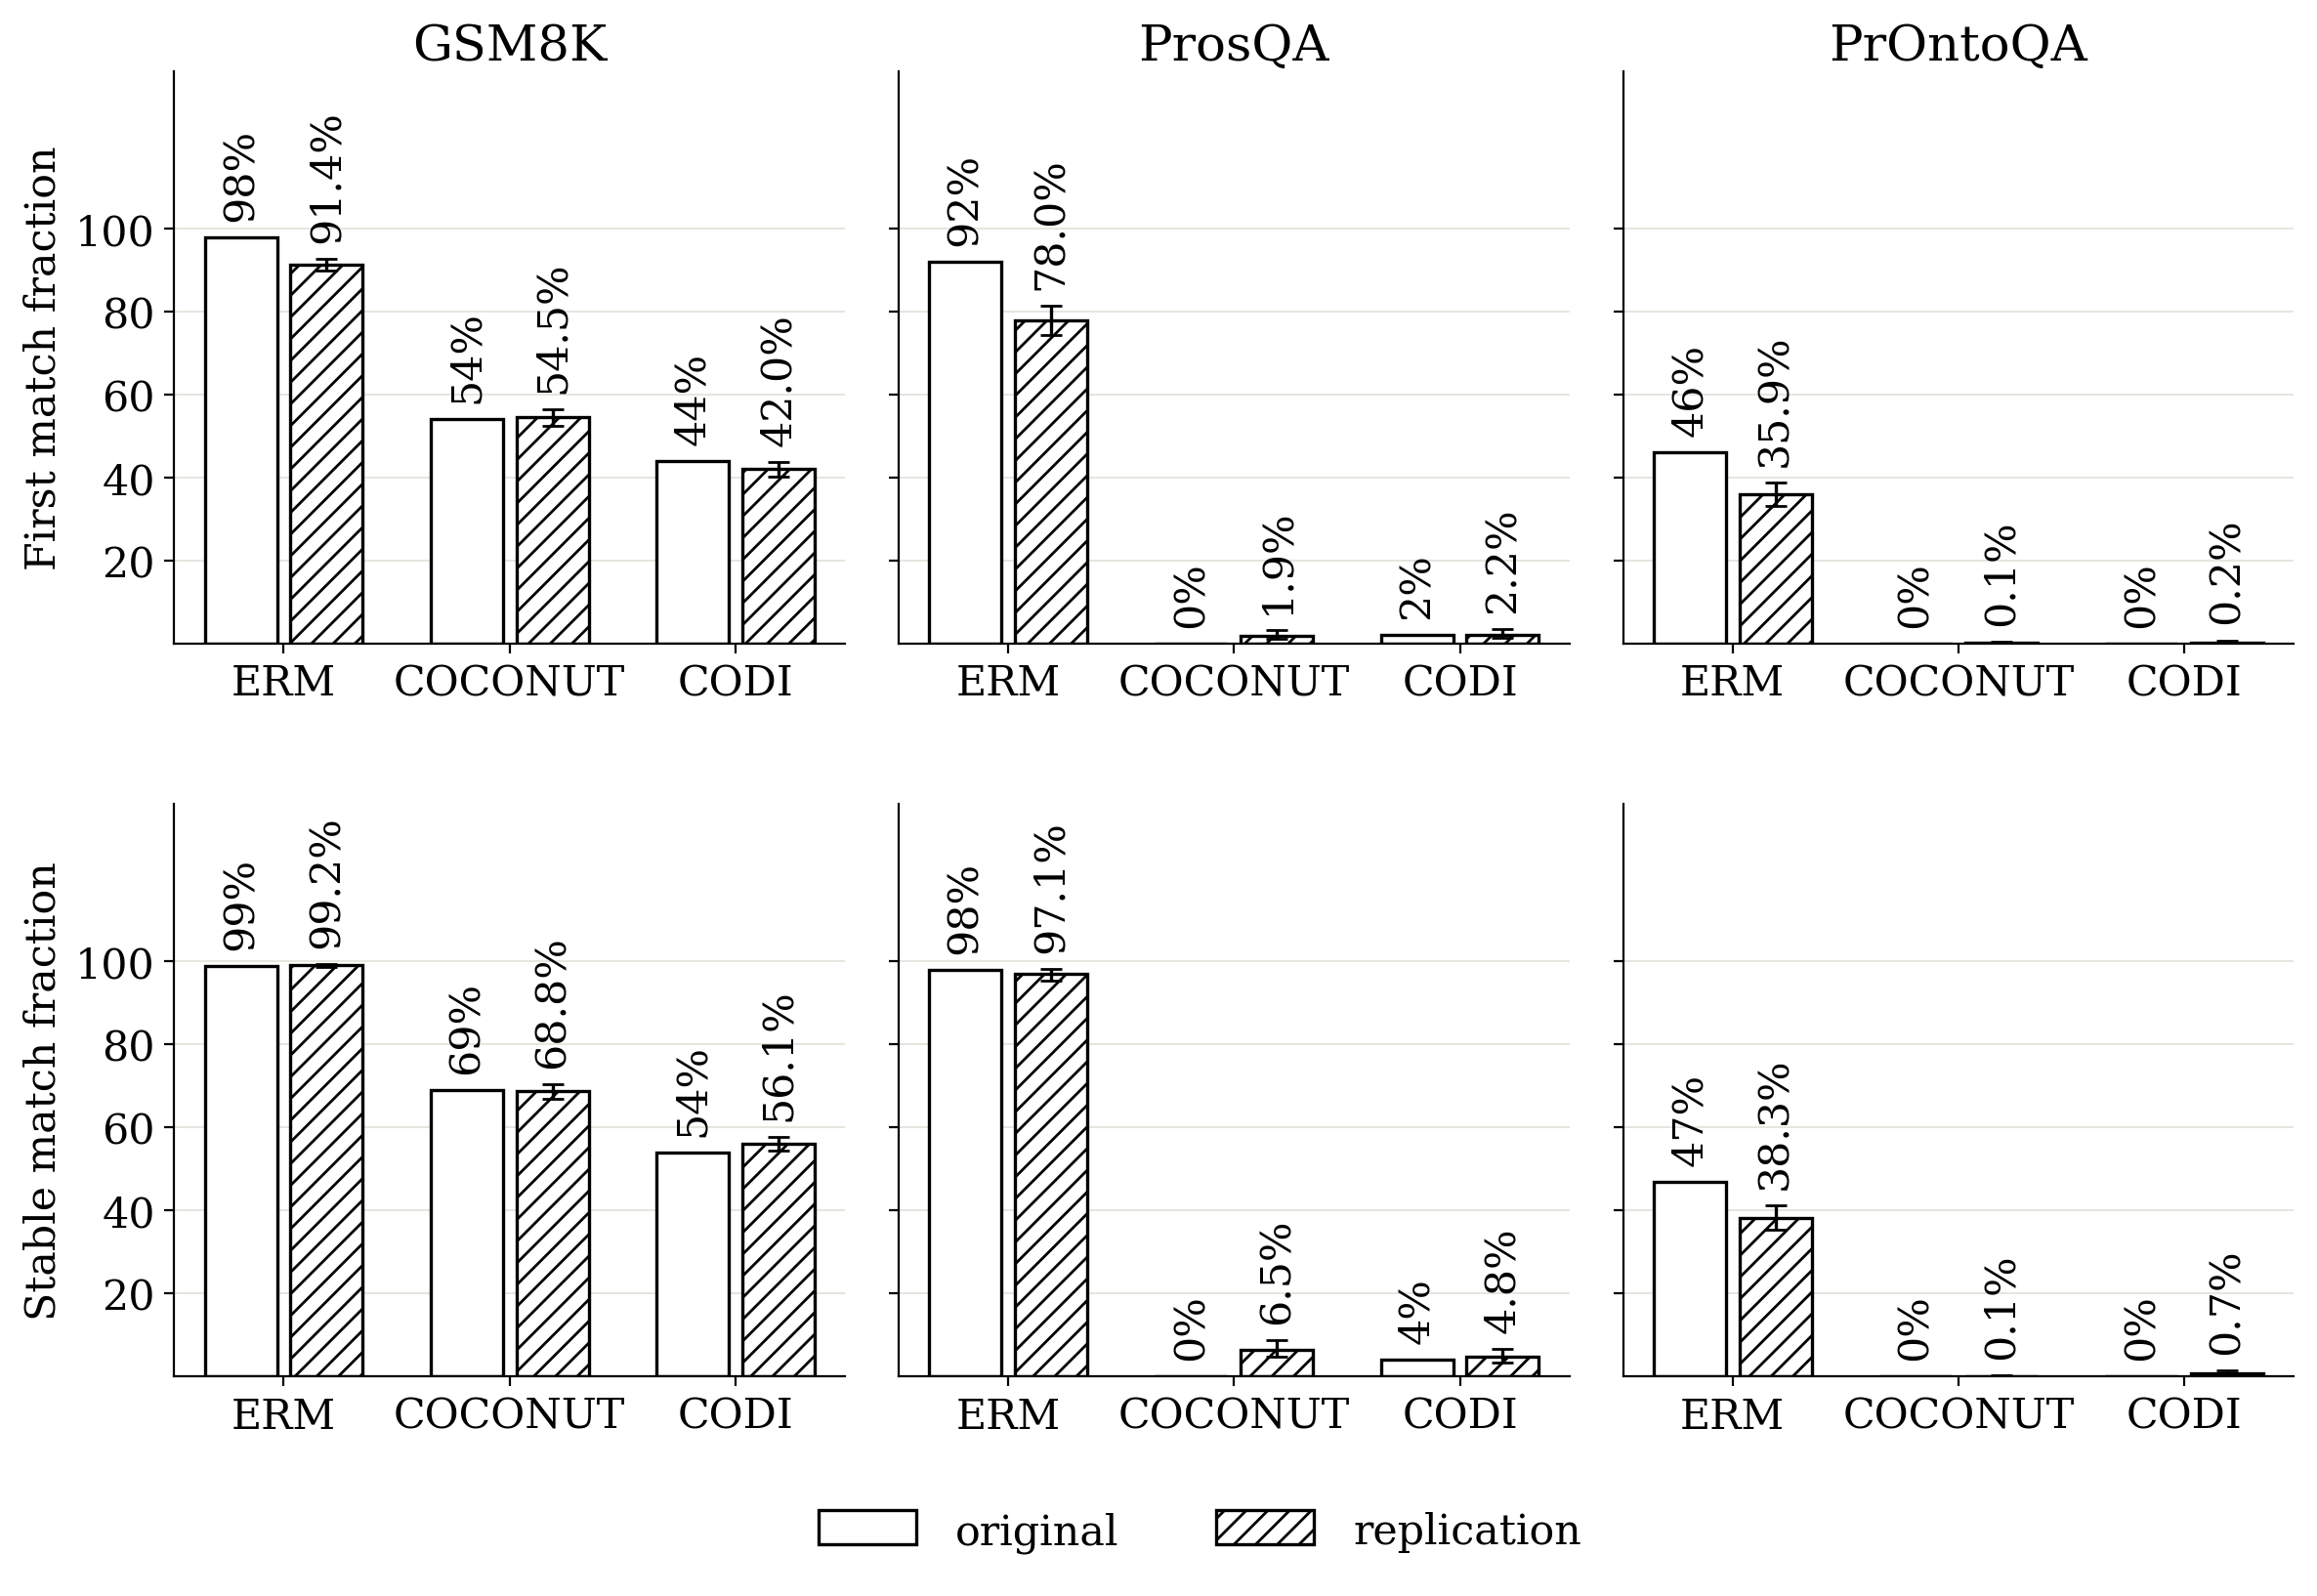
\includegraphics[width=\textwidth]{replication_grid.png}
  \caption {\textbf{Our reproduction produces similar \emph{first match} and \emph{stable match} scores as \citet{dilgren2026latent}.} Error bars on the reproduction bars are a 95\% bias-corrected and accelerated (BCa) bootstrap confidence interval (10,000 resamples) over the per-question first/stable match fractions; no comparable interval is available for the originally reported numbers, since only a single summary figure was published for each.}
  \label{fig:replication}
\end{figure*}

\begin{figure*}[]
  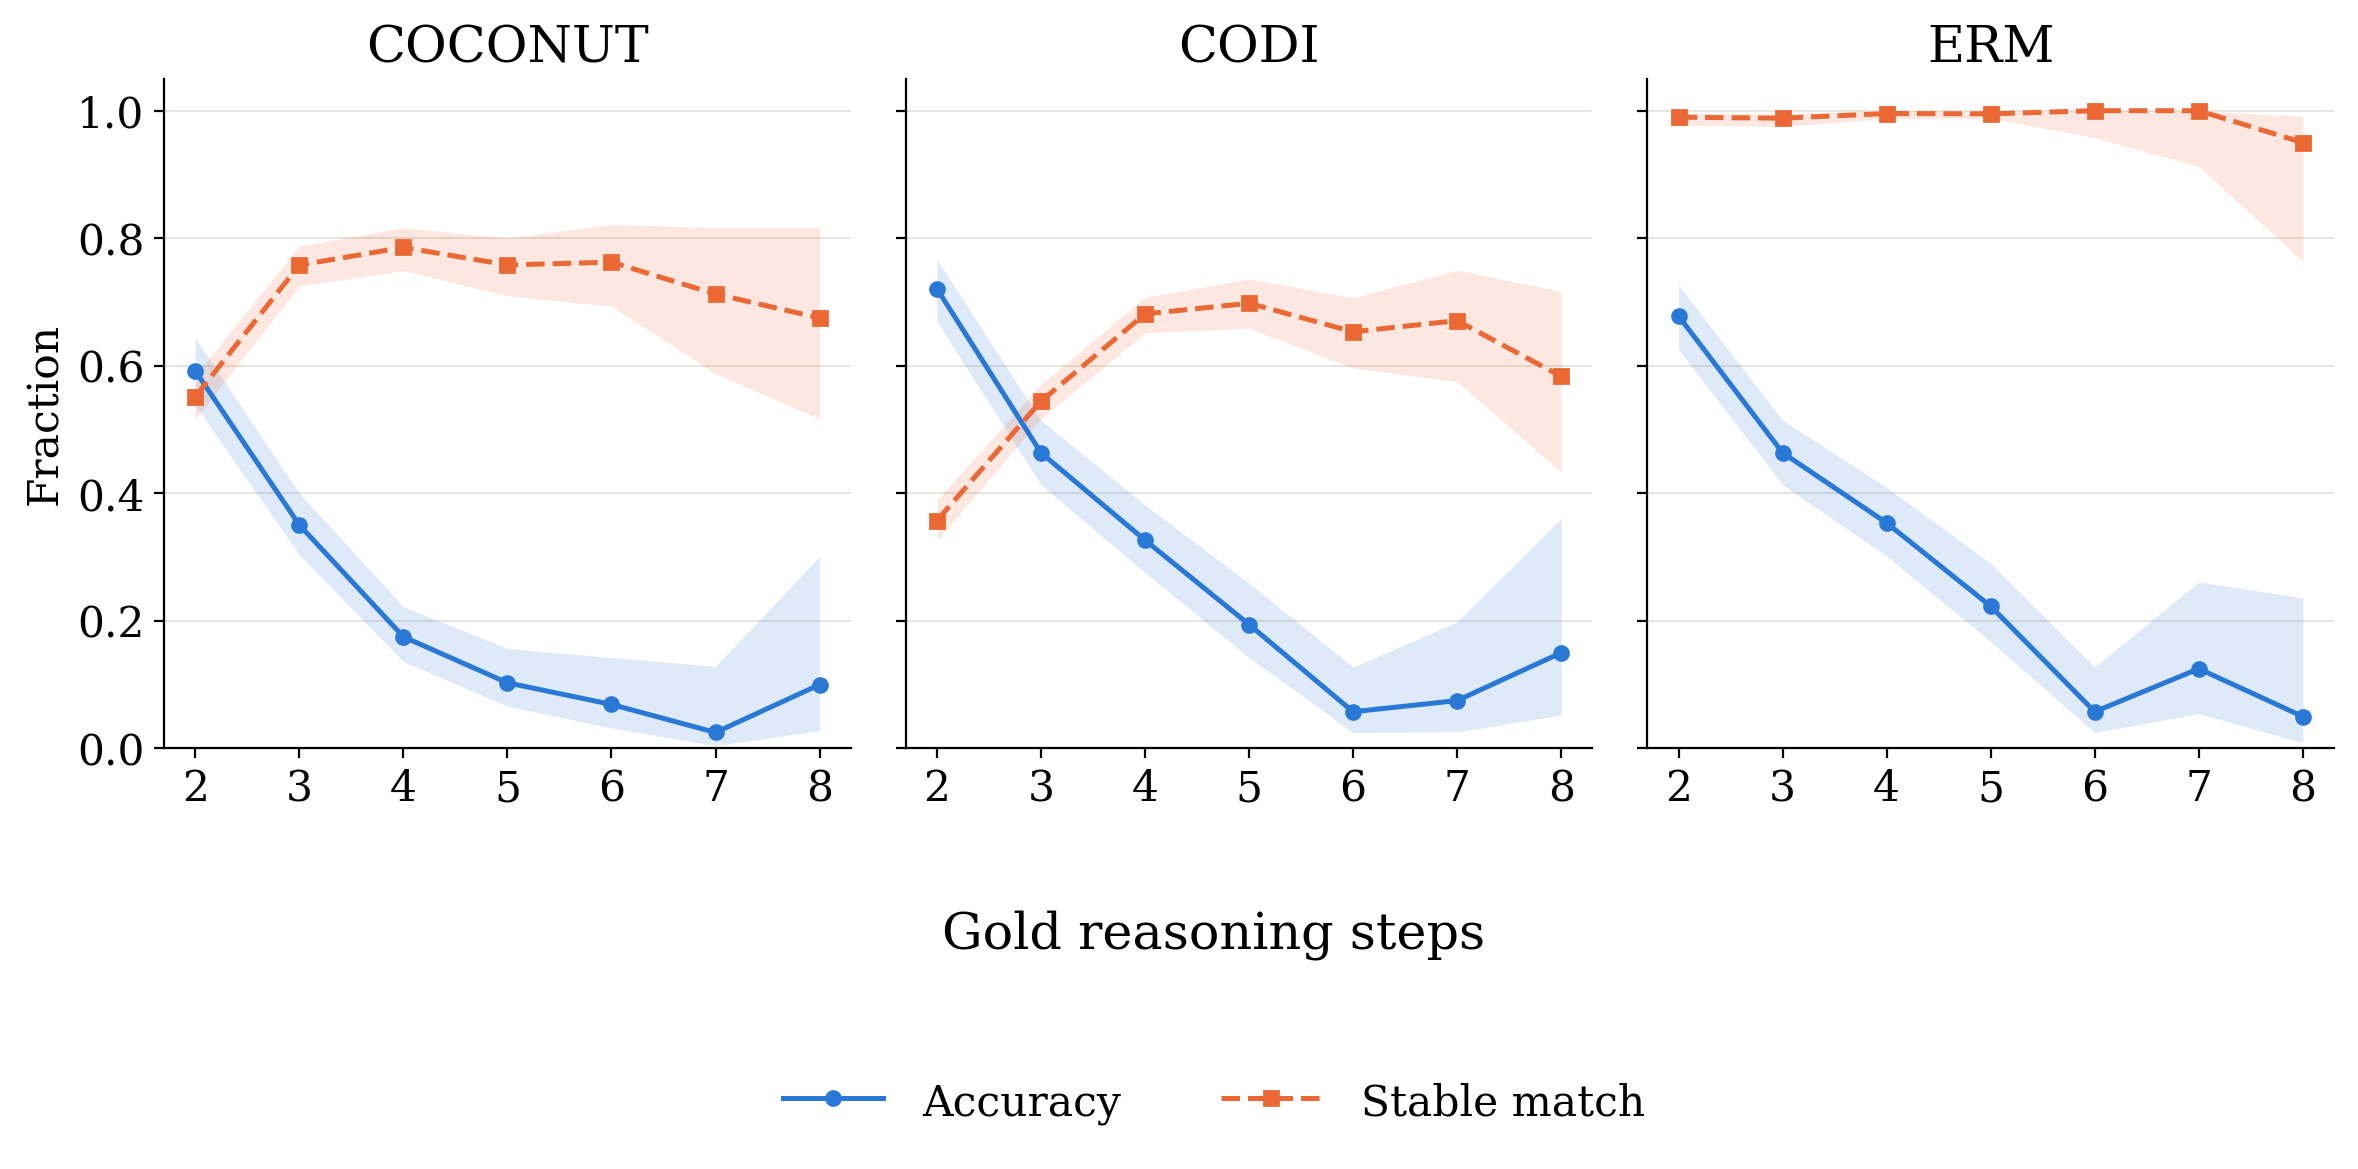
\includegraphics[width=\textwidth]{gold_steps_grid.png}
  \caption{\textbf{Testing accuracy and stable match score with increasing gold reasoning steps (GSM8k).}
  Shaded region is 95\% confidence interval: a Wilson score interval for accuracy, since it is a binomial correct/incorrect proportion; and a BCa bootstrap confidence interval (10,000 resamples) over per-question stable match fractions for stable match. As number of steps increases task difficulty is increased, as shown by reduced performance, and, in COCONUT and CODI, stable match increases.}
  \label{fig:steps}
\end{figure*}

\section{Fixed Token Budgets Produce Redundant Reasoning}
\label{sec:difficulty}

\citet{dilgren2026latent} propose two hypotheses that may explain why COCONUT and CODI produce lower matching metrics than the ERM: the first is that low task difficulty may cause matching metrics to be low in COCONUT and CODI, but not the ERM; the second is that COCONUT and CODI under-utilise their reasoning tokens relative to the ERM. Our results in this section support the first hypothesis, since we find that the LRM's matching metrics are affected substantially by task difficulty, \textit{i.e.,} they are lower on less difficult tasks, while the ERM's matching metrics are not, as shown in \Cref{fig:steps}. We proceed by refining the second hypothesis: we suggest that COCONUT and CODI may generate a similar number of effective reasoning steps as the ERM, as shown in Figure~\ref{fig:effective}, but they also generate additional redundant reasoning steps on simple questions to fill their fixed reasoning token budget.

\paragraph{Task Difficulty Is Associated With Stable Match} We bucket GSM8k samples by the number of computational steps represented with calculator notation in the gold reasoning trace. \Cref{fig:steps} shows that as the number of steps in a sample's gold reasoning trace increases, the accuracy of all three models decreases -- validating step count as a proxy for task difficulty. On the other hand LRMs' stable match fraction tends to increase, while the ERM's stable match fraction remains close to saturated.

\paragraph{Fixed Budgets Force Redundant Tokens} Figure~\ref{fig:effective} shows that all three models generate a similar number of effective reasoning steps, which means that lower stable match scores in the LRMs are the result of additional redundant reasoning tokens. We suggest that the LRMs generate these redundant tokens because, unlike the ERM, they have a fixed reasoning token budget. Simple questions may require fewer tokens than the budget permits, and residual tokens may not affect the model's answer.

\paragraph{ProsQA and PrOntoQA} We repeat this analysis on ProsQA (Appendix~\ref{sec:prosqa_bucket}); PrOntoQA is excluded because every exemplar trace contains exactly six steps, yielding a single bucket. ProsQA proves to be a degenerate case for this analysis: accuracy is flat across buckets for all three models, so gold step count does not track difficulty on this dataset, and the LRMs' stable match sits near zero in every bucket -- consistent with the fixed-budget account, under which uniformly easy problems render the whole latent budget redundant. Correspondingly, stable match diverges across models on ProsQA: the LRMs' falls near zero, while the ERM's approaches its full CoT length, which \Cref{sec:copying} suggests partly reflects its copying bias rather than additional computation.

\begin{figure}[h]
  \centering
  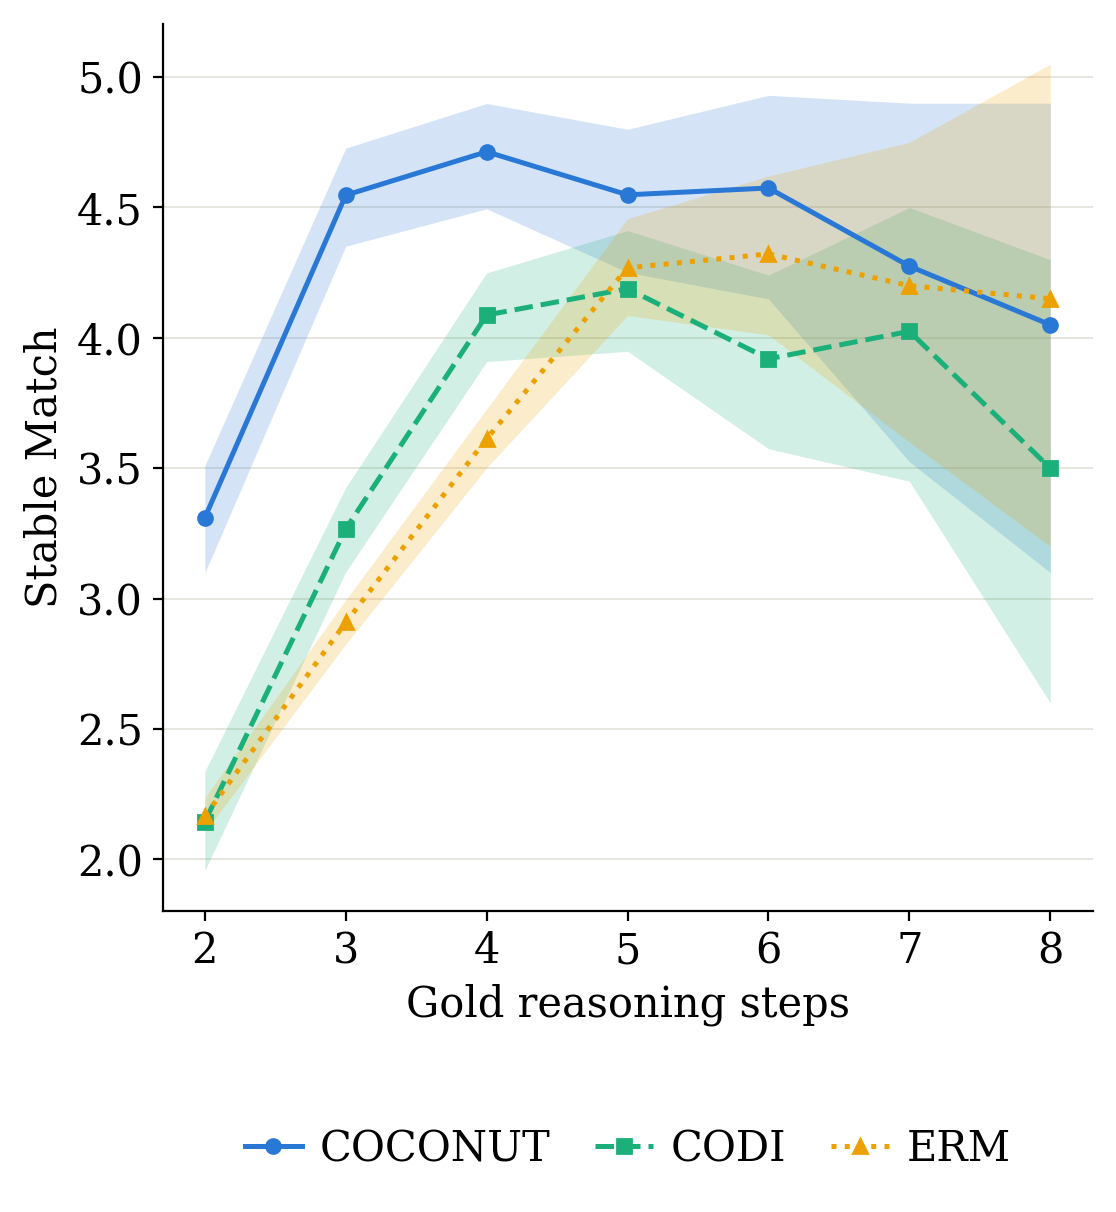
\includegraphics[width=\columnwidth]{effective_steps_by_gold_steps.png}
  \caption{\textbf{Effective reasoning steps of three models with increasing gold reasoning steps (GSM8k).} 
  All three models emit a similar number of effective reasoning steps on GSM8k questions with a given number of steps in the gold reasoning trace. Shaded regions are a 95\% BCa bootstrap confidence interval (10,000 resamples) over per-question effective-step values.}
  \label{fig:effective}
\end{figure}

\section{ERM's Answers May Be Copied From the Last Reasoning Step}
\label{sec:copying}

In this section we investigate whether the ERM has a tendency to copy the result of the last reasoning step when generating answers. This behaviour could account for some of the discrepancy in matching metrics between the LRMs and the ERM, since it could cause the ERM to change its answer each time the CoT is truncated.

\paragraph{Experimental Setup:} Each question in a given dataset is augmented. Then, each model is applied to both the original question, and the augmented variant. The resulting explicit reasoning steps and latent reasoning tokens are recorded. We proceed by running each model on the original question with truncated reasoning traces, as in Section~\ref{sec:experiment}. Before the model answers, we swap the last explicit reasoning step or latent reasoning token with the corresponding reasoning tokens generated for the augmented question.

\paragraph{Datasets:} We perform this experiment on both GSM8k and ProsQA. PrOntoQA is left for future work. GSM8k questions are augmented by swapping the first number in a problem statement with a random integer within the same order of magnitude. ProsQA questions are augmented by swapping every occurrence of two words throughout the problem statement. Specifically, question endings are of the form ``Is \textsc{name} a \textsc{opt1} or \textsc{opt2}?''. We identify which of \textsc{opt1}/\textsc{opt2} is correct (\emph{target}) and which is not (\emph{neg\_target}), then swap every occurrence of these two words throughout the question -- in every ``Every $Y$ is a $Z$.'' rule as well as the query itself. Because this is a pure relabelling of two symbols, any derivation chain that previously concluded \emph{target} now concludes \emph{neg\_target} and vice versa, so the correct answer is guaranteed to flip while every rule in the question remains logically valid.

\paragraph{Exclusion Criteria:} We exclude samples where: 1) a different number of explicit reasoning steps were produced for the original question and the augmented question, 2) the GSM8k question did not contain a number that could be perturbed, 3) the model gave the same answer to both questions at a given degree of CoT truncation, and 4) the model's last reasoning step was not effective. More details on excluded samples is available in Appendix~\ref{sec:appendix-exclusion}.

\paragraph{Answer Categorisation:} Answers are categorised as \emph{augmented}, if the swap causes the model's answer to match the answer given to the augmented question, \emph{original} if the swap resulted in no change, or \emph{other} if the resulting answer no longer matched either the original answer or the augmented one.

\paragraph{Results:} In \Cref{fig:copy-effective} and \Cref{fig:copy-effective-prosqa} we see that the ERM changes its answer substantially more often than either LRM, suggesting that the LRMs do not have an analogous copying bias to the ERM.

% We find that 64\% of the answers generated by the ERM while running the early stopping experiment on GSM8k were the same as the result of the preceding explicit reasoning step. We note that this includes answers that were generated while the CoT was truncated.

% We also run a variation of the early stopping experiment: before the model generates an answer we swap the result of the last explicit reasoning step with a random number within the same order of magnitude. When running this variation, the ERM's final answer matches this injected random number in 45.9\% of cases. It should be noted that in most cases, the random number has no plausible connection to the question. These results suggest that the ERM may have a tendency to copy the result of the last explicit reasoning reasoning step when generating an answer. However, this bias would only increase ERM's matching metrics relative to those of the LRMs if the LRMs did not have similar biases. 

% \begin{figure}[h]
%   \centering
%   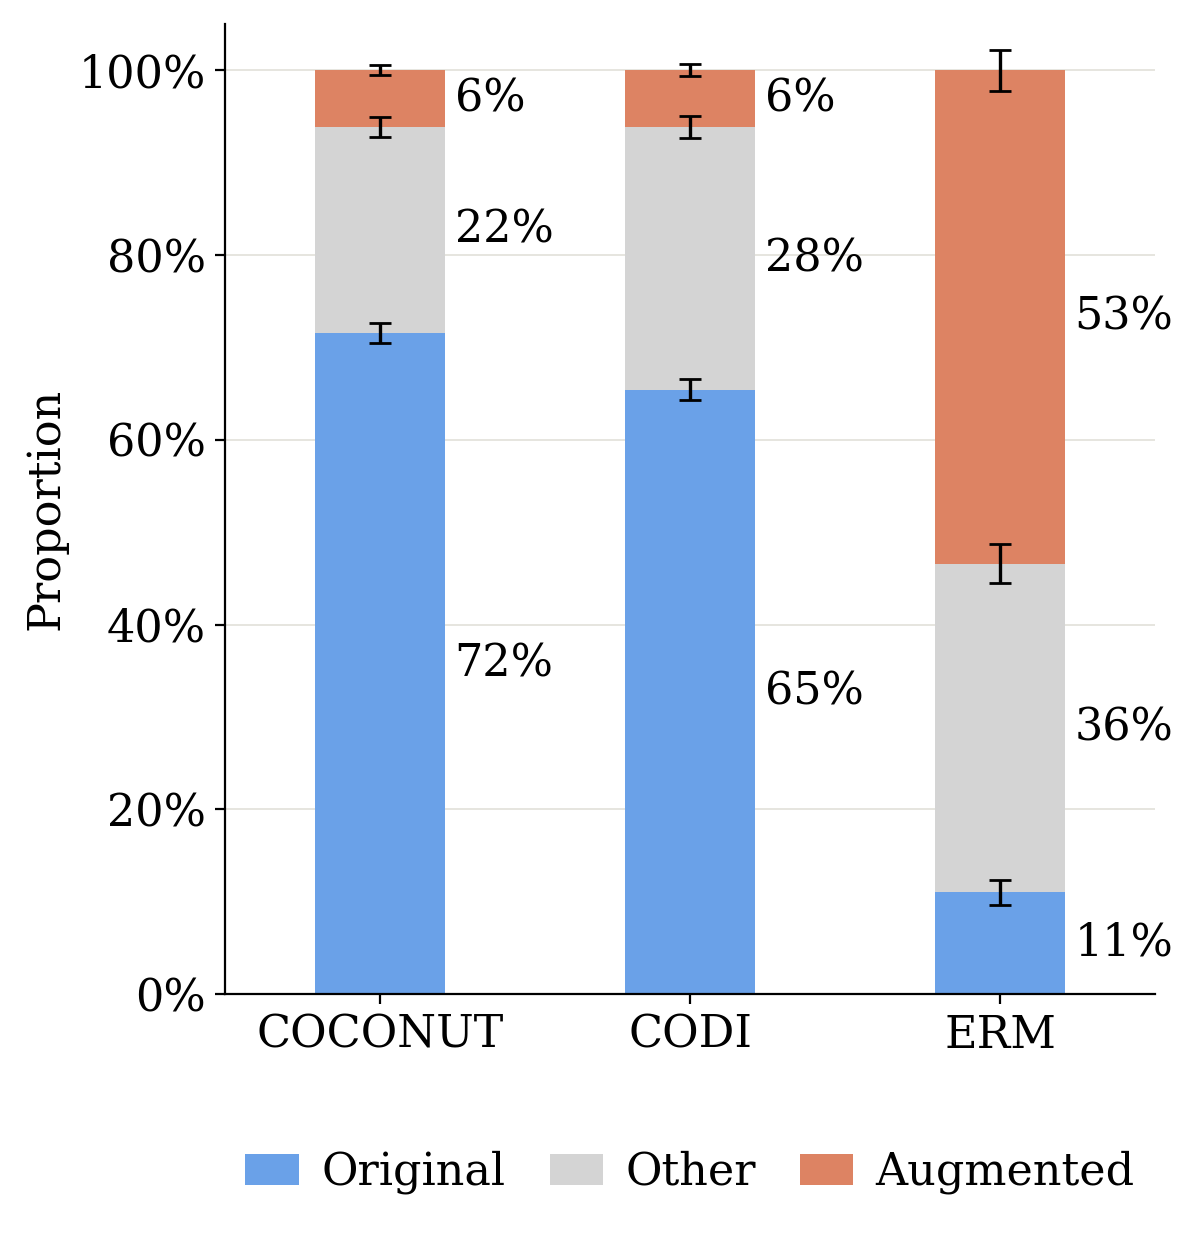
\includegraphics[width=\columnwidth]{slicing_status.png}
%   \caption{\textbf{Answer status after splicing one augmented-question reasoning step into an otherwise-original trace (GSM8k).} The resulting answer either still matches the original question (\emph{original}), switches to match the augmented question (\emph{augmented}), matches neither (\emph{other}). The ERM switches to the augmented answer far more often than COCONUT or CODI, consistent with a copying bias. Error bars are a 95\% cluster bootstrap confidence interval (10,000 resamples): whole questions, rather than individual steps, are resampled with replacement, since steps from the same question are correlated rather than independent trials.}
%   \label{fig:copy}
% \end{figure}

% Answer status after splicing, restricted to splices into an effective reasoning step (GSM8k).} As \Cref{fig:copy}, but dropping splicing trials at steps that could not have changed the model's answer -- steps at or after the point where the unperturbed trace's own answer had already stabilized (\Cref{fig:effective}), so swapping in the augmented step there tests nothing. The same pattern survives this restriction: the ERM still switches to the augmented answer far more often than COCONUT or CODI.

\begin{figure}[h]
  \centering
  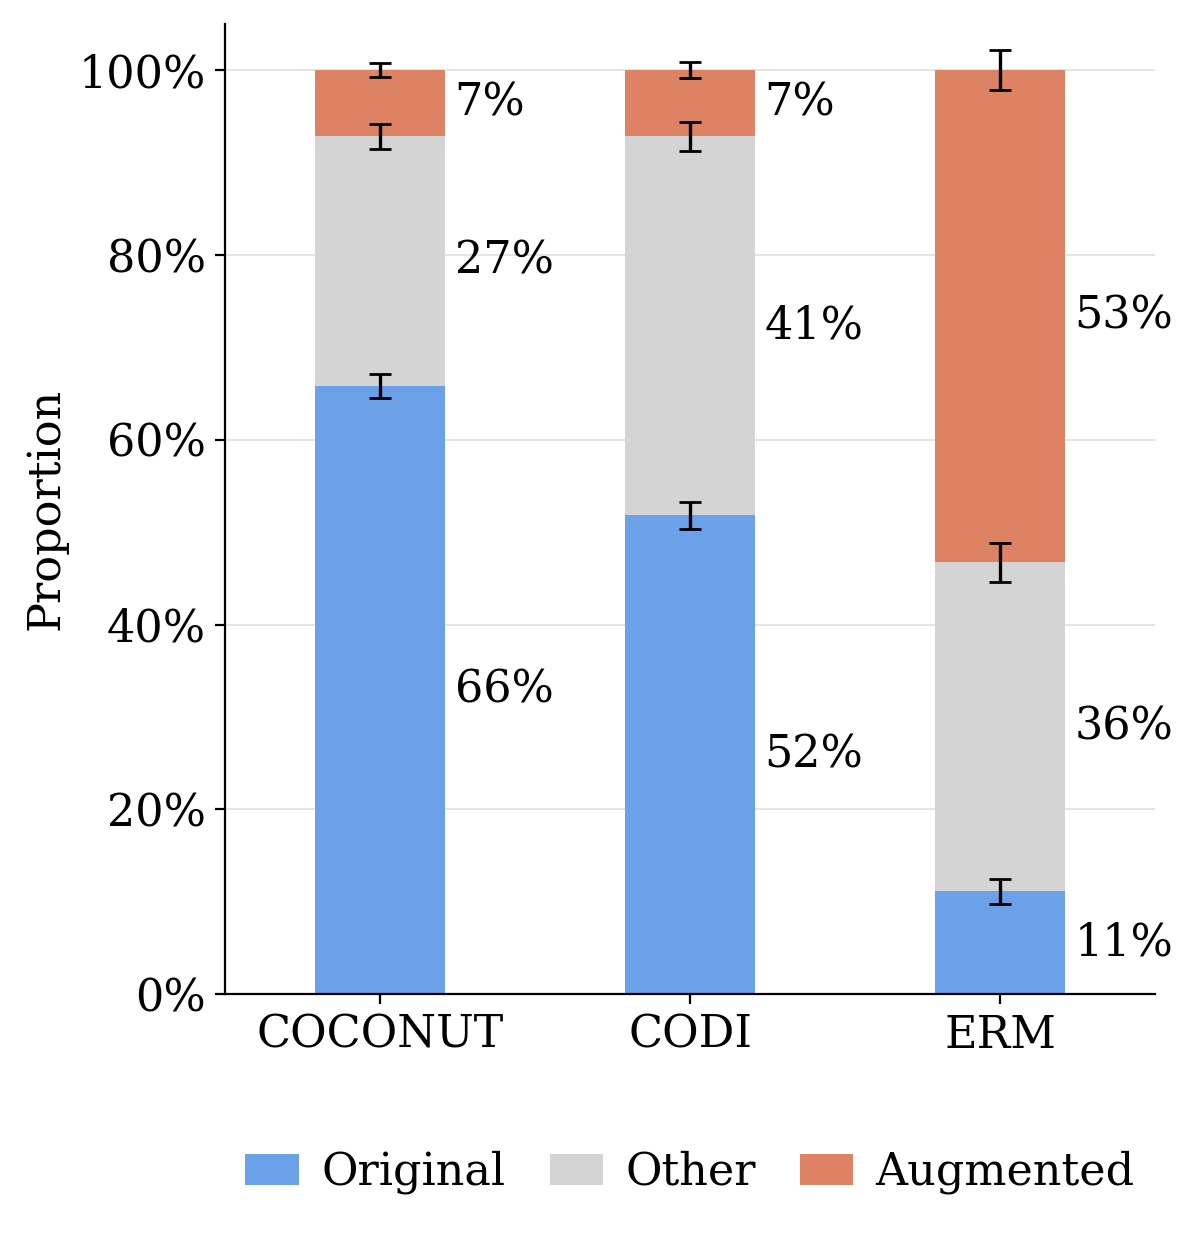
\includegraphics[width=\columnwidth]{slicing_status_effective.png}
  \caption{\textbf{Answer status after splicing one augmented-question reasoning step into an otherwise-original trace (GSM8k).} The resulting answer either still matches the original question (\emph{original}), switches to match the augmented question (\emph{augmented}), matches neither (\emph{other}). The ERM switches to the augmented answer far more often than COCONUT or CODI, consistent with a copying bias. Error bars are a 95\% cluster bootstrap confidence interval (10,000 resamples): whole questions, rather than individual steps, are resampled with replacement, since steps from the same question are correlated rather than independent trials.}
  \label{fig:copy-effective}
\end{figure}

% \begin{figure}[h]
%   \centering
%   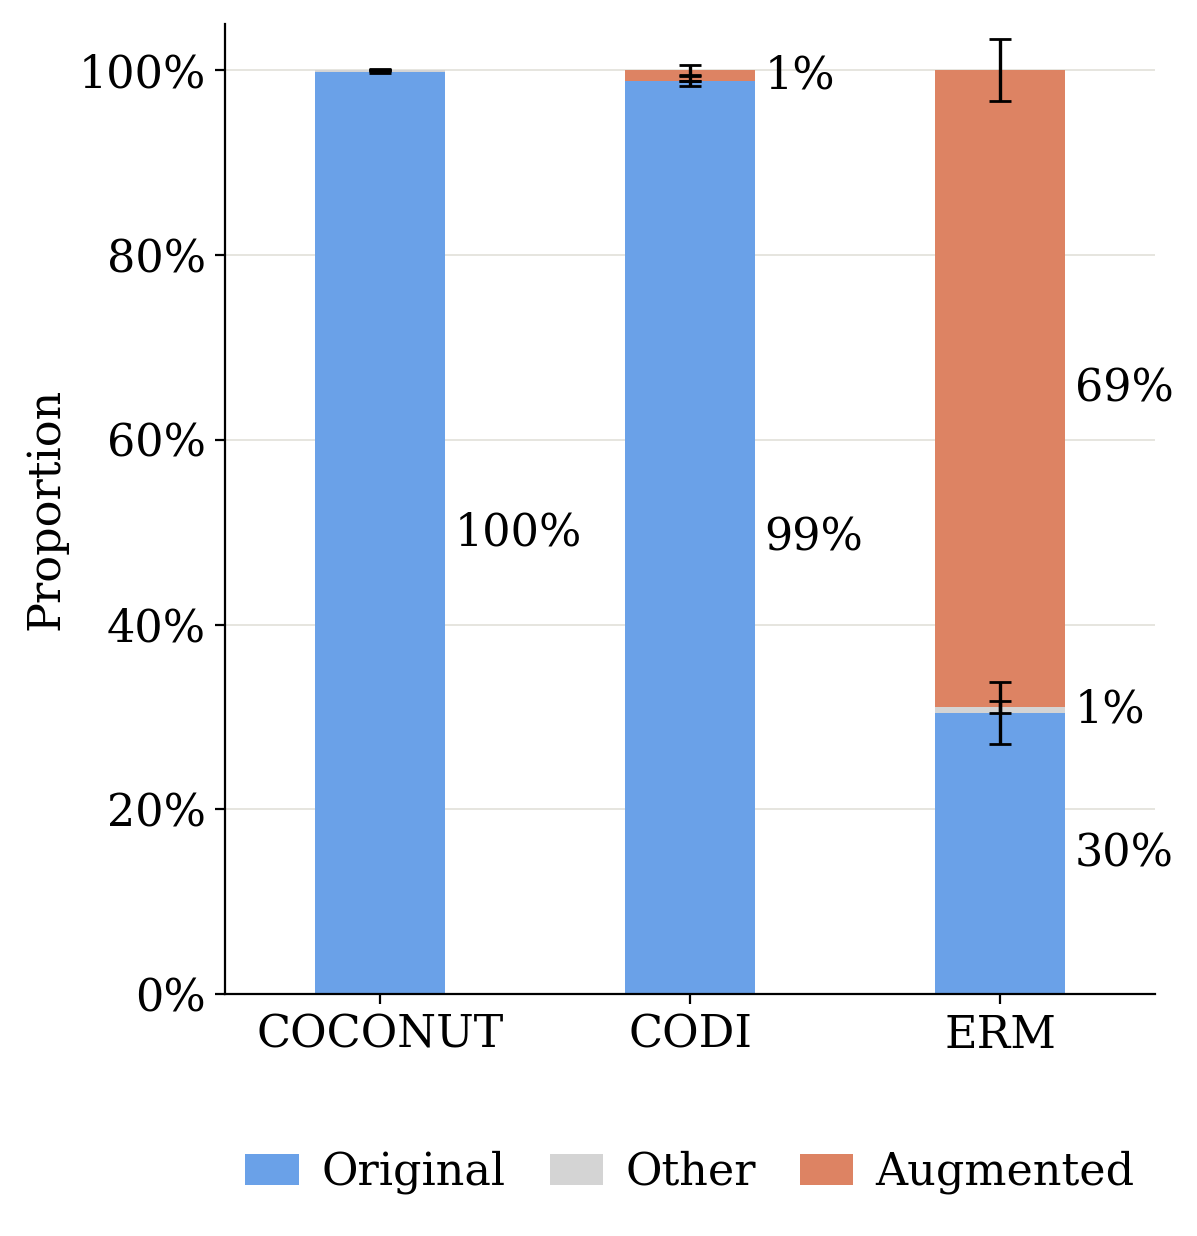
\includegraphics[width=\columnwidth]{slicing_status_prosqa.png}
%   \caption{\textbf{Answer status after splicing one augmented-question reasoning step into an otherwise-original trace (ProsQA).} As \Cref{fig:copy}, but with the augmented question built by swapping the query's two named class options everywhere they appear (see text). The ERM switches to the augmented answer far more often than COCONUT or CODI, consistent with \Cref{fig:copy}. Error bars are a 95\% cluster bootstrap confidence interval (10,000 resamples) over whole questions.}
%   \label{fig:copy-prosqa}
% \end{figure}

% Answer status after splicing, restricted to splices into an effective reasoning step (ProsQA).} As \Cref{fig:copy-effective}, restricting \Cref{fig:copy-prosqa} to splices at steps before the unperturbed trace's own answer had stabilized. COCONUT's proportions barely move, but CODI's augmented share rises to 32\% (from 1.1\% unrestricted) -- still well short of the ERM's 69\%, but showing CODI is more sensitive to the swapped content than the pooled figure alone suggests.

\begin{figure}[h]
  \centering
  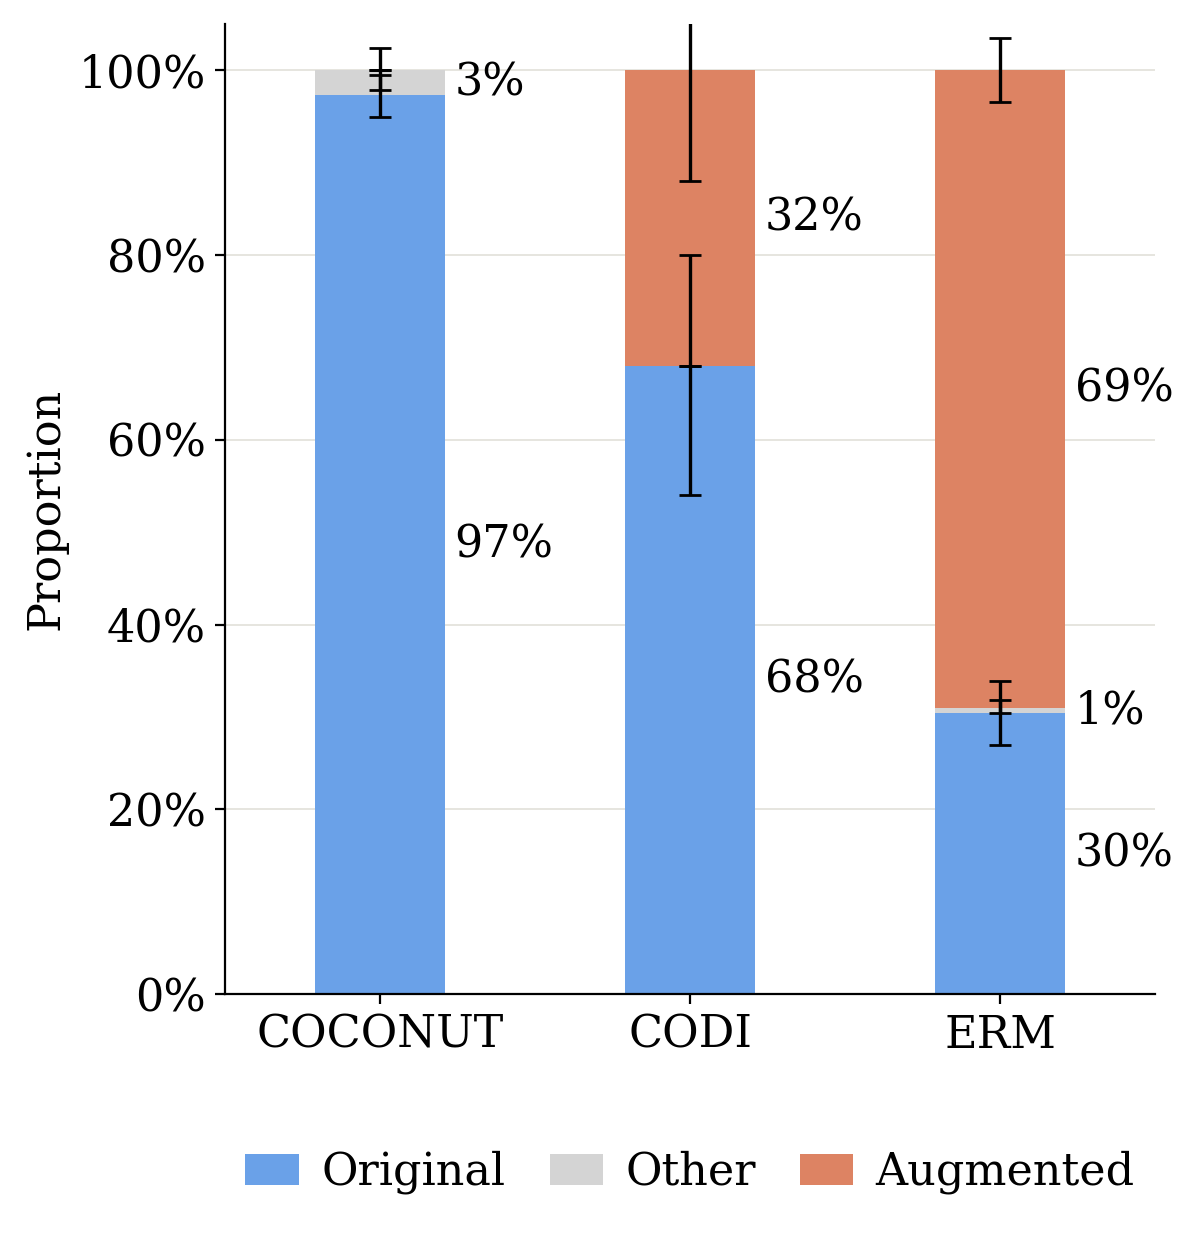
\includegraphics[width=\columnwidth]{slicing_status_effective_prosqa.png}
  \caption{\textbf{Answer status after splicing one augmented-question reasoning step into an otherwise-original trace (ProsQA).} As \Cref{fig:copy-effective}, but with the augmented question built by swapping the query's two named class options everywhere they appear (see text). The ERM switches to the augmented answer far more often than COCONUT or CODI, consistent with \Cref{fig:copy-effective}. Error bars are a 95\% cluster bootstrap confidence interval (10,000 resamples) over whole questions.}
  \label{fig:copy-effective-prosqa}
\end{figure}

\if 0
\section{Limitations}
%todo{jx:is "Limitations" section mandatory for this submission? otherwise, we can remove it as it really weakens our current work and conclusions. I agree this section either needs removing or extending considerably to do it justice. I think that give the nature of the paper removing it is the best option, but if it's essential then I understand given our limited time.}

The experiments referred to in \Cref{sec:difficulty} and \Cref{sec:copying} were not done on ProsQA or PrOntoQA, so we cannot be certain that the factors identified in this paper generalise to those domains.
\fi

\section{Conclusion}

In this paper, we successfully reproduce the results of \citet{dilgren2026latent}, and design targeted experiments to identify two factors that may explain the gap in matching metrics between the ERM, and the LRMs (COCONUT and CODI). First, fixed token budgets force latent reasoning models to generate redundant tokens, thereby reducing their matching metrics relative to the ERM. Second, the ERM has a tendency to copy the result of the most recent explicit reasoning step when generating its final answer, thereby increasing its matching metrics relative to the LRMs. These findings refine the hypothesis that COCONUT and CODI under-utilise their latent reasoning tokens. Instead, we conclude that they effectively use tokens early in the CoT \citep{chang_unlocking_2026}, the number of which varies with problem complexity. Furthermore, our results suggest that truncation-based evaluations of CoT necessity, and faithfulness tests built on the same operation \citep{lanham2023measuring}, are sensitive to the way in which a model uses its CoT. We suggest that future work investigates whether our evaluations of model faithfulness can be influenced by whether the model explores multiple candidate solutions in its CoT, and by where key results appear within the model's CoT.


% \section{Engines}

% To produce a PDF file, pdf\LaTeX{} is strongly recommended (over original \LaTeX{} plus dvips+ps2pdf or dvipdf).
% The style file \texttt{acl.sty} can also be used with
% lua\LaTeX{} and
% Xe\LaTeX{}, which are especially suitable for text in non-Latin scripts.
% The file \texttt{acl\_lualatex.tex} in this repository provides
% an example of how to use \texttt{acl.sty} with either
% lua\LaTeX{} or
% Xe\LaTeX{}.

% \section{Preamble}

% The first line of the file must be
% \begin{quote}
% \begin{verbatim}
% \documentclass[11pt]{article}
% \end{verbatim}
% \end{quote}

% To load the style file in the review version:
% \begin{quote}
% \begin{verbatim}
% \usepackage[review]{acl}
% \end{verbatim}
% \end{quote}
% For the final version, omit the \verb|review| option:
% \begin{quote}
% \begin{verbatim}
% \usepackage{acl}
% \end{verbatim}
% \end{quote}

% To use Times Roman, put the following in the preamble:
% \begin{quote}
% \begin{verbatim}
% \usepackage{times}
% \end{verbatim}
% \end{quote}
% (Alternatives like txfonts or newtx are also acceptable.)

% Please see the \LaTeX{} source of this document for comments on other packages that may be useful.

% Set the title and author using \verb|\title| and \verb|\author|. Within the author list, format multiple authors using \verb|\and| and \verb|\And| and \verb|\AND|; please see the \LaTeX{} source for examples.

% By default, the box containing the title and author names is set to the minimum of 5 cm. If you need more space, include the following in the preamble:
% \begin{quote}
% \begin{verbatim}
% \setlength\titlebox{<dim>}
% \end{verbatim}
% \end{quote}
% where \verb|<dim>| is replaced with a length. Do not set this length smaller than 5 cm.

% \section{Document Body}

% \subsection{Footnotes}

% Footnotes are inserted with the \verb|\footnote| command.\footnote{This is a footnote.}

% \subsection{Tables and figures}

% See Table~\ref{tab:accents} for an example of a table and its caption.
% \textbf{Do not override the default caption sizes.}

% \begin{table}
%   \centering
%   \begin{tabular}{lc}
%     \hline
%     \textbf{Command} & \textbf{Output} \\
%     \hline
%     \verb|{\"a}|     & {\"a}           \\
%     \verb|{\^e}|     & {\^e}           \\
%     \verb|{\`i}|     & {\`i}           \\
%     \verb|{\.I}|     & {\.I}           \\
%     \verb|{\o}|      & {\o}            \\
%     \verb|{\'u}|     & {\'u}           \\
%     \verb|{\aa}|     & {\aa}           \\\hline
%   \end{tabular}
%   \begin{tabular}{lc}
%     \hline
%     \textbf{Command} & \textbf{Output} \\
%     \hline
%     \verb|{\c c}|    & {\c c}          \\
%     \verb|{\u g}|    & {\u g}          \\
%     \verb|{\l}|      & {\l}            \\
%     \verb|{\~n}|     & {\~n}           \\
%     \verb|{\H o}|    & {\H o}          \\
%     \verb|{\v r}|    & {\v r}          \\
%     \verb|{\ss}|     & {\ss}           \\
%     \hline
%   \end{tabular}
%   \caption{Example commands for accented characters, to be used in, \emph{e.g.}, Bib\TeX{} entries.}
%   \label{tab:accents}
% \end{table}

% As much as possible, fonts in figures should conform
% to the document fonts. See Figure~\ref{fig:experiments} for an example of a figure and its caption.

% Using the \verb|graphicx| package graphics files can be included within figure
% environment at an appropriate point within the text.
% The \verb|graphicx| package supports various optional arguments to control the
% appearance of the figure.
% You must include it explicitly in the \LaTeX{} preamble (after the
% \verb|\documentclass| declaration and before \verb|\begin{document}|) using
% \verb|\usepackage{graphicx}|.

% \begin{figure}[t]
%   \includegraphics[width=\columnwidth]{example-image-golden}
%   \caption{A figure with a caption that runs for more than one line.
%     Example image is usually available through the \texttt{mwe} package
%     without even mentioning it in the preamble.}
%   \label{fig:experiments}
% \end{figure}

% \begin{figure*}[t]
%   \includegraphics[width=0.48\linewidth]{example-image-a} \hfill
%   \includegraphics[width=0.48\linewidth]{example-image-b}
%   \caption {A minimal working example to demonstrate how to place
%     two images side-by-side.}
% \end{figure*}

% \subsection{Hyperlinks}

% Users of older versions of \LaTeX{} may encounter the following error during compilation:
% \begin{quote}
% \verb|\pdfendlink| ended up in different nesting level than \verb|\pdfstartlink|.
% \end{quote}
% This happens when pdf\LaTeX{} is used and a citation splits across a page boundary. The best way to fix this is to upgrade \LaTeX{} to 2018-12-01 or later.

% \subsection{Citations}

% \begin{table*}
%   \centering
%   \begin{tabular}{lll}
%     \hline
%     \textbf{Output}           & \textbf{natbib command} & \textbf{ACL only command} \\
%     \hline
%     \citep{Gusfield:97}       & \verb|\citep|           &                           \\
%     \citealp{Gusfield:97}     & \verb|\citealp|         &                           \\
%     \citet{Gusfield:97}       & \verb|\citet|           &                           \\
%     \citeyearpar{Gusfield:97} & \verb|\citeyearpar|     &                           \\
%     \citeposs{Gusfield:97}    &                         & \verb|\citeposs|          \\
%     \hline
%   \end{tabular}
%   \caption{\label{citation-guide}
%     Citation commands supported by the style file.
%     The style is based on the natbib package and supports all natbib citation commands.
%     It also supports commands defined in previous ACL style files for compatibility.
%   }
% \end{table*}

% Table~\ref{citation-guide} shows the syntax supported by the style files.
% We encourage you to use the natbib styles.
% You can use the command \verb|\citet| (cite in text) to get ``author (year)'' citations, like this citation to a paper by \citet{Gusfield:97}.
% You can use the command \verb|\citep| (cite in parentheses) to get ``(author, year)'' citations \citep{Gusfield:97}.
% You can use the command \verb|\citealp| (alternative cite without parentheses) to get ``author, year'' citations, which is useful for using citations within parentheses (e.g. \citealp{Gusfield:97}).

% A possessive citation can be made with the command \verb|\citeposs|.
% This is not a standard natbib command, so it is generally not compatible
% with other style files.

% \subsection{References}

% \nocite{Ando2005,andrew2007scalable,rasooli-tetrault-2015}

% The \LaTeX{} and Bib\TeX{} style files provided roughly follow the American Psychological Association format.
% If your own bib file is named \texttt{custom.bib}, then placing the following before any appendices in your \LaTeX{} file will generate the references section for you:
% \begin{quote}
% \begin{verbatim}
% \bibliography{custom}
% \end{verbatim}
% \end{quote}

% You can obtain the complete ACL Anthology as a Bib\TeX{} file from \url{https://aclweb.org/anthology/anthology.bib.gz}.
% To include both the Anthology and your own .bib file, use the following instead of the above.
% \begin{quote}
% \begin{verbatim}
% \bibliography{anthology,custom}
% \end{verbatim}
% \end{quote}

% Please see Section~\ref{sec:bibtex} for information on preparing Bib\TeX{} files.

% \subsection{Equations}

% An example equation is shown below:
% \begin{equation}
%   \label{eq:example}
%   A = \pi r^2
% \end{equation}

% Labels for equation numbers, sections, subsections, figures and tables
% are all defined with the \verb|\label{label}| command and cross references
% to them are made with the \verb|\ref{label}| command.

% This an example cross-reference to Equation~\ref{eq:example}.

% \subsection{Appendices}

% Use \verb|\appendix| before any appendix section to switch the section numbering over to letters. See Appendix~\ref{sec:appendix} for an example.

% \section{Bib\TeX{} Files}
% \label{sec:bibtex}

% Unicode cannot be used in Bib\TeX{} entries, and some ways of typing special characters can disrupt Bib\TeX's alphabetization. The recommended way of typing special characters is shown in Table~\ref{tab:accents}.

% Please ensure that Bib\TeX{} records contain DOIs or URLs when possible, and for all the ACL materials that you reference.
% Use the \verb|doi| field for DOIs and the \verb|url| field for URLs.
% If a Bib\TeX{} entry has a URL or DOI field, the paper title in the references section will appear as a hyperlink to the paper, using the hyperref \LaTeX{} package.

% \section*{Limitations}

% This document does not cover the content requirements for ACL or any
% other specific venue.  Check the author instructions for
% information on
% maximum page lengths, the required ``Limitations'' section,
% and so on.

% Uncomment in camera ready!
% \section*{Acknowledgments}

% This work was supported by UKRI AI Centre for Doctoral Training in Safe Artificial Intelligence Systems (SAINTS) (EP/Y030540/1)

% Bibliography entries for the entire Anthology, followed by custom entries
%\bibliography{anthology,custom}
% Custom bibliography entries only
\bibliography{custom}

\appendix

\section{Dataset Examples}
\label{sec:appendix-examples}

We give one representative test-split instance from each dataset used in our experiments (\Cref{sec:experiment}), chosen among the shorter instances in each dataset for space. GSM8k's gold answer is a natural-language reasoning trace with numerical operations annotated in calculator notation (\Cref{sec:experiment}); ProsQA and PrOntoQA instead provide their gold reasoning as an explicit list of steps, with a short final answer.

\subsection{GSM8K}

\paragraph{Question:} An eraser costs \$2 and a pencil costs \$3. How much do 6 erasers and 8 pencils cost?

\paragraph{Gold answer:}
\begin{quote}
Six erasers cost \$2/eraser x 6 erasers = \$\verb|<<2*6=12>>|12.
Eight pencils cost \$3/pencil x 8 pencils = \$\verb|<<3*8=24>>|24.
So, 6 erasers and 8 pencils cost \$12 + \$24 = \$36.
\#\#\#\# 36
\end{quote}

\subsection{ProsQA}

\paragraph{Question:} Every zumpus is a timpus. Every jompus is a terpus. Eva is a sterpus. Eva is a zumpus. Max is a rorpus. Every timpus is a lorpus. Every jompus is a rorpus. Every tumpus is a terpus. Every sterpus is a zumpus. Every terpus is a gerpus. Tom is a storpus. Every zumpus is a jompus. Every sterpus is a timpus. Every storpus is a boompus. Tom is a boompus. Every timpus is a tumpus. Is Eva a boompus or gerpus?

\paragraph{Gold reasoning steps:}
\begin{enumerate}
\item Eva is a zumpus.
\item Every zumpus is a jompus.
\item Every jompus is a terpus.
\item Every terpus is a gerpus.
\end{enumerate}

\paragraph{Answer:} Eva is a gerpus.

\subsection{PrOntoQA}

\textbf{Question:} Grimpuses are angry. Jompuses are lempuses. Zumpuses are earthy. Grimpuses are jompuses. Every gorpus is not hot. Jompuses are moderate. Zumpuses are dumpuses. Each lorpus is not spicy. Shumpuses are dull. Lempuses are yumpuses. Tumpuses are sterpuses. Wumpuses are shy. Lempuses are wumpuses. Each yumpus is opaque. Yumpuses are tumpuses. Lempuses are not small. Tumpuses are impuses. Yumpuses are vumpuses. Tumpuses are not dull. Sterpuses are discordant. Vumpuses are brown. Grimpuses are gorpuses. Jompuses are lorpuses. Rex is a zumpus. Rex is a grimpus. True or false: Rex is dull.

\paragraph{Gold reasoning steps:}
\begin{enumerate}
\item Rex is a grimpus. Grimpuses are jompuses.
\item Rex is a jompus. Jompuses are lempuses.
\item Rex is a lempus. Lempuses are yumpuses.
\item Rex is a yumpus. Yumpuses are tumpuses.
\item Rex is a tumpus. Tumpuses are not dull.
\item Rex is not dull.
\end{enumerate}

\paragraph{Answer:} False

\section{Dataset Splits}
\label{sec:appendix-splits}

\Cref{tab:splits} gives the train/validation/test split sizes for each dataset used in our experiments (\Cref{sec:experiment}). All of our own evaluation is run on the test split only, using models already fine-tuned by the original authors; we did not do any training ourselves. GSM8K's splits come from its standard Hugging Face Hub mirror (\texttt{openai/gsm8k}), which does not define a validation split. ProsQA and PrOntoQA's splits come from the replicated paper's own repository (\Cref{sec:experiment}).

\begin{table}[h]
\centering
\small
\begin{tabular}{lrrr}
\toprule
Dataset & Train & Valid & Test \\
\midrule
GSM8K & 7{,}473 & --- & 1{,}319 \\
ProsQA & 17{,}886 & 300 & 500 \\
PrOntoQA & 9{,}000 & 200 & 800 \\
\bottomrule
\end{tabular}
\caption{Number of instances in each split, by dataset.}
\label{tab:splits}
\end{table}

\section{Bucketing ProsQA by Steps}
\label{sec:prosqa_bucket}

\Cref{sec:difficulty} repeats the GSM8k gold-step-count bucketing analysis (\Cref{fig:steps}) on ProsQA, bucketing each test sample by the length of its gold reasoning chain (\Cref{sec:appendix-examples}) rather than by calculator-notation steps. \Cref{fig:steps-prosqa} shows the result: unlike on GSM8k, accuracy does not decrease as gold step count increases for any of the three models, so step count is not a difficulty signal on this dataset. COCONUT and CODI's stable match stays near zero across every bucket, while the ERM's stays near its maximum -- the same divergence seen on GSM8k, but without the step-count trend that on GSM8k ties it to task difficulty. 

\begin{figure*}[]
  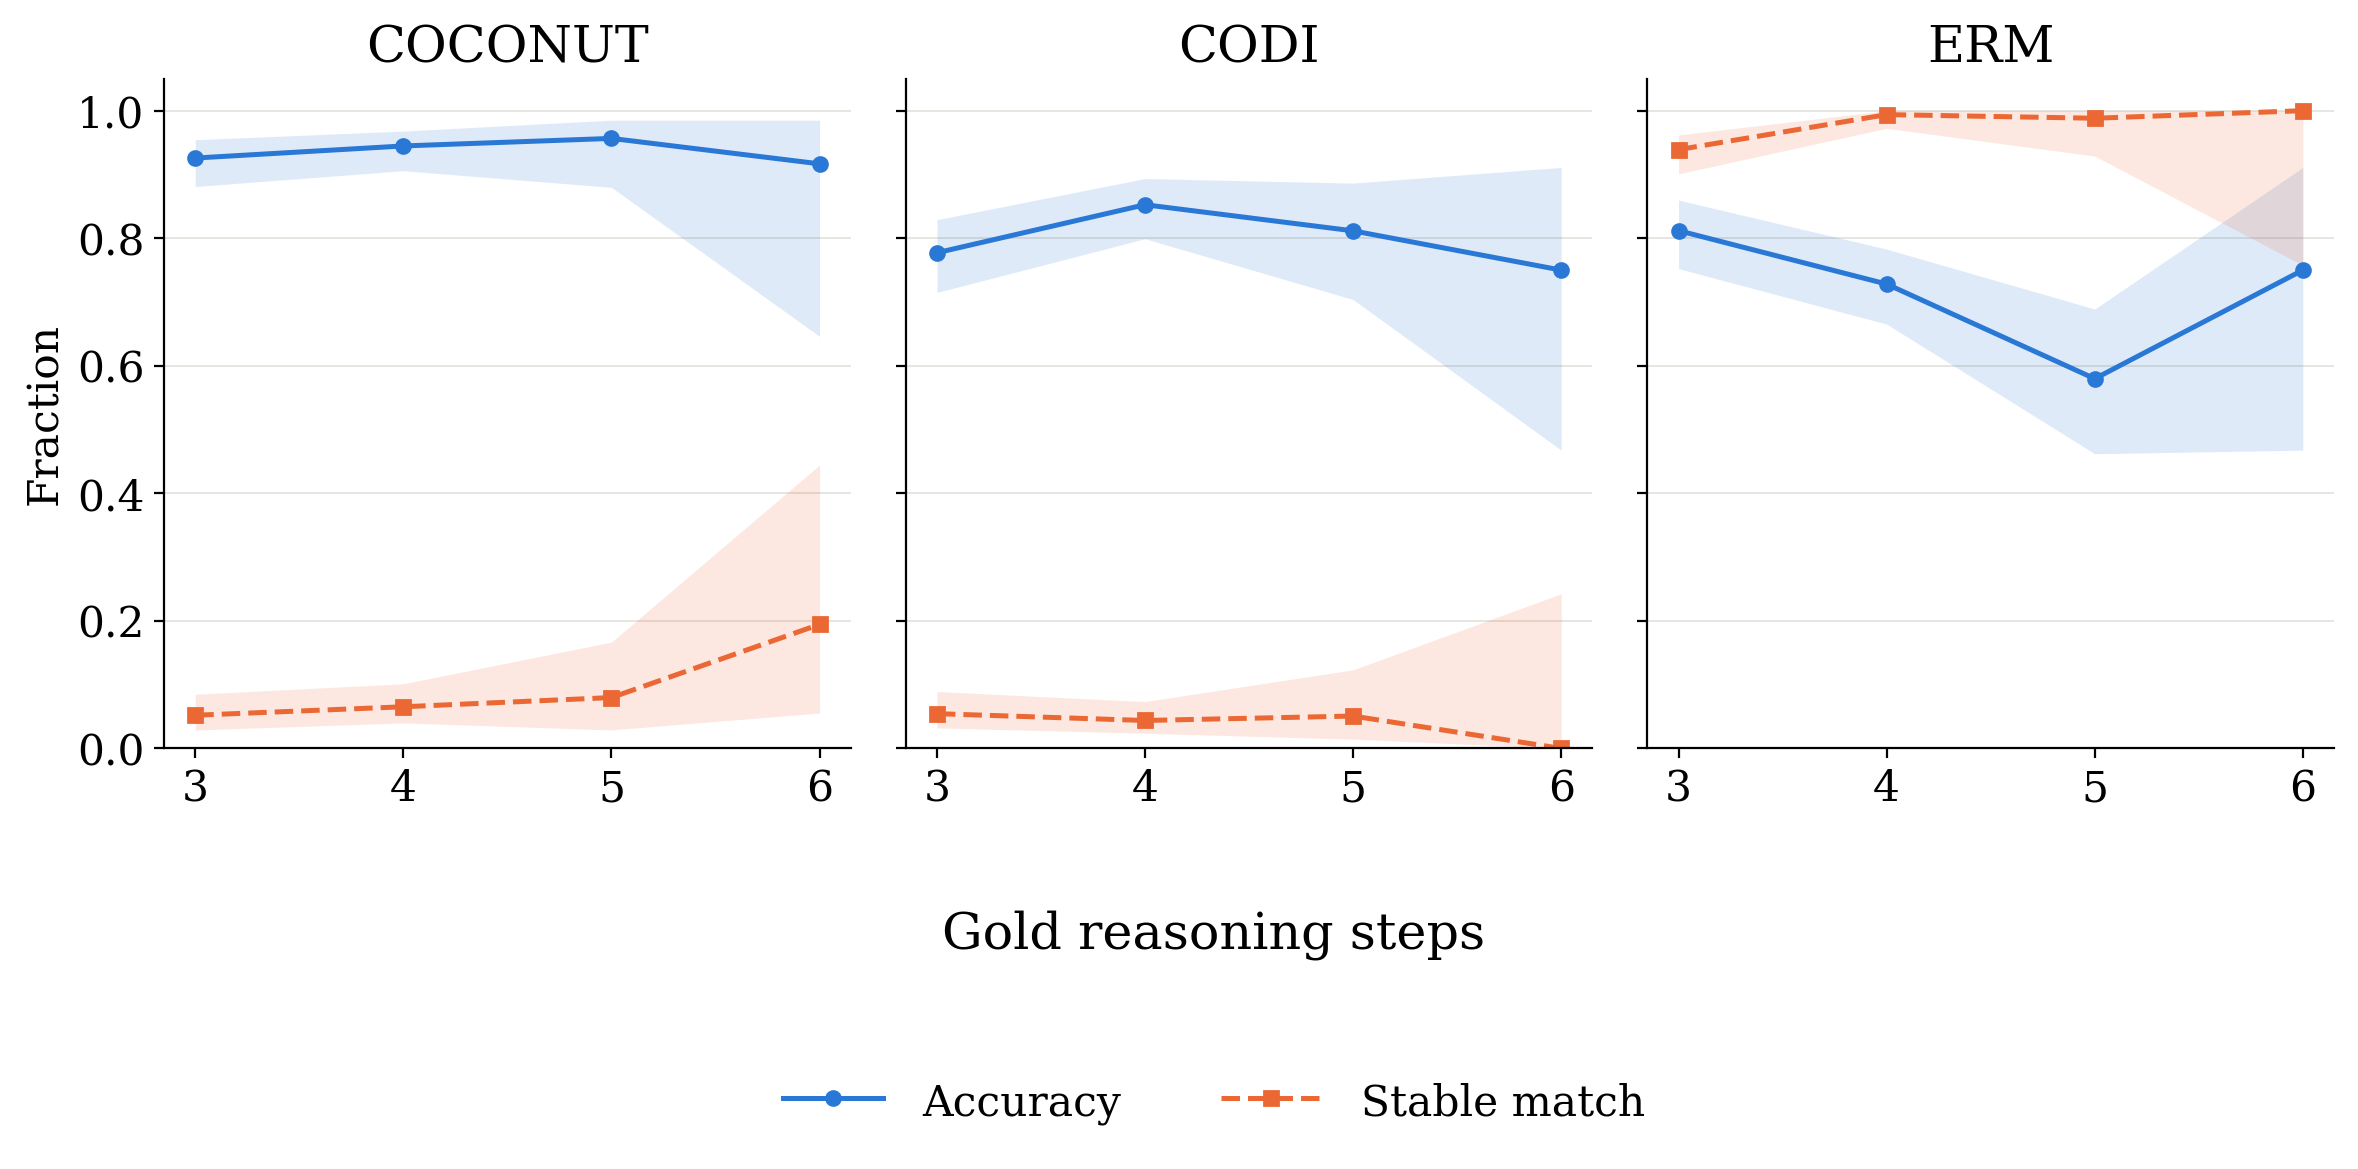
\includegraphics[width=\textwidth]{gold_steps_grid_prosqa.png}
  \caption{\textbf{Testing accuracy and stable match score with increasing gold reasoning steps (ProsQA).} As \Cref{fig:steps}, but bucketed by the length of each sample's gold reasoning chain instead of calculator-notation steps. Shaded region is a 95\% confidence interval: a Wilson score interval for accuracy, and a BCa bootstrap confidence interval (10,000 resamples) over per-question stable match fractions for stable match. Accuracy is roughly flat across buckets for all three models, and COCONUT and CODI's stable match remains near zero throughout, in contrast to the GSM8k trend in \Cref{fig:steps}.}
  \label{fig:steps-prosqa}
\end{figure*}

\section{Sample Exclusion for the Copying-Bias Experiment}
\label{sec:appendix-exclusion}

\Cref{sec:copying} excludes some GSM8k test samples from the copying-bias slicing experiment (\Cref{fig:copy-effective}) before computing each model's \emph{original}, \emph{augmented}, and \emph{other} proportions. \Cref{tab:exclusion} shows how many of the 1,319 GSM8k test samples remain for each model after these exclusions. A third criterion mentioned in \Cref{sec:copying} entails excluding cases where the model gives the same answer to the original and augmented questions at a given degree of CoT truncation. We label these cases as \emph{Ties}, and show the remaining sample counts in \Cref{tab:exclusion-trials}. \Cref{tab:exclusion-prosqa,tab:exclusion-trials-prosqa} give the same breakdown for the ProsQA version of this experiment (\Cref{fig:copy-effective-prosqa}).

\begin{table}[h]
\centering
\small
\begin{tabular}{lrrr}
\toprule
Model & No number & Step mismatch & Remaining \\
\midrule
ERM      & 23 & 353 & 943 \\
COCONUT  & 23 & --- & 1{,}296 \\
CODI     & 23 & --- & 1{,}296 \\
\bottomrule
\end{tabular}
\caption{GSM8k test samples excluded from the copying-bias slicing experiment (\Cref{fig:copy-effective}), out of 1,319 total, and the number remaining. ``No number'': the question contains no number that can be perturbed to build an augmented question. ``Step mismatch'': the original and augmented questions produced a different number of explicit reasoning steps (ERM only).}
\label{tab:exclusion}
\end{table}

\begin{table}[h]
\centering
\small
\begin{tabular}{lrrr}
\toprule
Model & Before & Ties & After \\
\midrule
ERM      & 2{,}876 & 640   & 2{,}236 \\
COCONUT  & 7{,}776 & 1{,}413 & 6{,}363 \\
CODI     & 7{,}776 & 802   & 6{,}974 \\
\bottomrule
\end{tabular}
\caption{Splicing trials underlying \Cref{fig:copy-effective}, summed over the remaining samples in \Cref{tab:exclusion}: total trials before removing ties, the number of those tagged \emph{tie}, and the number of non-tie trials remaining, which is what \Cref{fig:copy-effective}'s \emph{original}/\emph{augmented}/\emph{other} proportions are computed over.}
\label{tab:exclusion-trials}
\end{table}

\begin{table}[h]
\centering
\small
\begin{tabular}{lrrr}
\toprule
Model & Unparseable & Step mismatch & Remaining \\
\midrule
ERM      & 0 & 83  & 417 \\
COCONUT  & 0 & --- & 500 \\
CODI     & 0 & --- & 500 \\
\bottomrule
\end{tabular}
\caption{ProsQA test samples excluded from the copying-bias slicing experiment (\Cref{fig:copy-effective-prosqa}), out of 500 total, and the number remaining.}
\label{tab:exclusion-prosqa}
\end{table}

\begin{table}[h]
\centering
\small
\begin{tabular}{lrrr}
\toprule
Model & Before & Ties & After \\
\midrule
ERM      & 1{,}613 & 1{,}078 & 535   \\
COCONUT  & 3{,}000 & 111     & 2{,}889 \\
CODI     & 3{,}000 & 549     & 2{,}451 \\
\bottomrule
\end{tabular}
\caption{Splicing trials underlying \Cref{fig:copy-effective-prosqa}, summed over the remaining samples in \Cref{tab:exclusion-prosqa}. Compared to \Cref{tab:exclusion-trials}, the ProsQA word-swap augmentation touches several rules per question rather than a single number, which leaves far fewer ties for COCONUT and CODI (and a correspondingly larger set of non-tie trials) than the GSM8k version of this experiment.}
\label{tab:exclusion-trials-prosqa}
\end{table}

\end{document}
